\documentclass[a4paper,fleqn,usenatbib]{mnras}

\usepackage{newtxtext,newtxmath}
% Depending on your LaTeX fonts installation, you might get better results with one of these:
%\usepackage{mathptmx}
%\usepackage{txfonts}

\usepackage[T1]{fontenc}
\usepackage{ae,aecompl}

\usepackage{numprint}
\usepackage{booktabs}
\usepackage{float}

\usepackage{amsbsy}
\usepackage{graphicx}	% Including figure files
\usepackage{color}
\usepackage{amsmath}	% Advanced maths commands
\usepackage{amssymb}	% Extra maths symbols

\newcommand{\todo}[1]{\textcolor{red}{#1}}

%%%%%%%%%%%%%%%%%%%%%%%%%%%%%%%%%%%%%%%%%%%%%%%%%%

%%%%% AUTHORS - PLACE YOUR OWN COMMANDS HERE %%%%%

% Please keep new commands to a minimum, and use \newcommand not \def to avoid
% overwriting existing commands. Example:
%\newcommand{\pcm}{\,cm$^{-2}$}	% per cm-squared

%%%%%%%%%%%%%%%%%%%%%%%%%%%%%%%%%%%%%%%%%%%%%%%%%%


% Title of the paper, and the short title which is used in the headers.
% Keep the title short and informative.
\title[Discovery of 47 r-process stars from the LAMOST survey]{Discovery of 47 $r$-process stars from the LAMOST survey}

% The list of authors, and the short list which is used in the headers.
% If you need two or more lines of authors, add an extra line using \newauthor
\author[Matthew T. Miles et al.]{Matthew T. Miles,$^{1}$\thanks{E-mail: mtmil3@student.monash.edu}
	Andrew R. Casey,$^{1,2}$
	Brodie J. Norfolk,$^{1}$
	Alex J. Kemp,$^{1}$\newauthor
	John C. Lattanzio,$^{1}$
	Kevin C. Schlaufman,$^{3}$
	Alexander P. Ji,$^{4}$
	Anna Y. Q. Ho,$^{5}$
	\\
	% List of institutions
	$^{1}$School of Physics and Astronomy, Monash University, Clayton Campus, Victoria 3800, Australia\\
	$^{2}$Faculty of Information Technology, Monash University, Clayton Campus, Victoria 3800, Australia\\
	$^{3}$Department of Physics and Astronomy, Johns Hopkins University, 3400 N Charles St., Baltimore, MD 21218, USA\\
	$^{4}$Department of Physics and Kavli Institute for Astrophysics and Space Research, Massachusetts Institute of Technology, Cambridge, MA 02139, USA\\
	$^{5}$Cahill Center for Astrophysics, California Institute of Technology, MC 249-17, 1200 E California Blvd, Pasadena, CA, 91125, USA
}

\date{Accepted XXX. Received YYY; in original form ZZZ}

\pubyear{2018}

\begin{document}
	\label{firstpage}
	\pagerange{\pageref{firstpage}--\pageref{lastpage}}
	\maketitle
	
	\begin{abstract}
		The production of heavy elements occurs through the slow and rapid neutron capture process. Numerous sites satisfy the conditions needed to synthesise r-process elements, but the frequency and abundance of these sites is unclear. The lack of a large number of stars with strong r-process signatures limits us. Here we report the discovery of 47 r-process enhanced stars from the LAMOST survey, more than doubling the known number in our Galaxy. Additionally, we provide the first estimate, to our knowledge, of whether neutron star mergers are able to account for the r-process element abundances in all known r-process enhanced stars in the Milky Way. The discovery of these stars implies multiple r-process sites, contrary to previous conclusions in the literature including all r-process material being produced in small amounts in common events such as core-collapse supernovae, or the material only being produced in very large amounts in very rare events, such as neutron star mergers. 
	\end{abstract}
	
	\begin{keywords}
		nucleosynthesis -- r-process -- neutron star mergers -- core-collapse supernovae
	\end{keywords}
	
	
	\section{Introduction}
	
	Heavy elements ($Z > 30$) are synthesised through the slow (s) and rapid (r) neutron capture processes \citep{Sneden2008}. The nucleosynthesis of these elements has been a key area in astrophysics research since it was first theorised  \citep{Burbidge1957}.
	
	For over 60 years theorists have argued about the potential sites of the r-process. The r-process occurs when the neutron density is high enough that the rate of neutron capture will occur faster than the rate at which the isotope undergoes a $\beta$-decay. The sites where this phenomena can occur are very specific, with the most favoured being core-collapse supernovae, neutron star mergers, or magnetorotationally driven supernovae. Core-collapse supernovae are relatively common throughout the Galaxy, but they only produce small amounts of r-process material. Neutron star mergers or magnetorotationally driven supernovae, however, occur much more infrequently than core-collapse supernovae, but produce far more r-process material. Events such as these are theorised to account for the case of the highly r-process enhanced ultra-faint dwarf (UFD) galaxy Reticulum II \citep{Ji2016}. Neutron star mergers may have a stronger argument to be the parent site of this level of r-process enhancement in such a small volume. However, magnetorotationally driven supernovae are also a possible solution.

	While magnetorotationally driven supernovae may not produce as much r-process material as neutron star mergers (although still more than core-collapse supernovae), they occur more frequently, and enough material is produced that it is currently impossible to distinguish between them through abundance signatures.
	
	Europium (Z=63), is entirely produced through the r-process. This makes it a very useful signature when detecting stars that show evidence of pollution by r-process material. The recent discovery of the UFD Reticulum II used Europium as evidence of its r-process enhancement, and found the particularly interesting result that the UFD's level of r-process enrichment was too high to have occurred through a core-collapse supernovae event.

	Historically UFD's have had some of the lowest abundance of r-process elements of any celestial body. However analysis of several of Reticulum II's stars show they are greatly enriched, 2-3 orders of magnitude higher than stars found in any other UFD galaxy \citep{Ji2016}. This degree of enrichment supports the theory that a single rare event must have occurred in the galaxies formative years to enrich it, as (for Europium especially) the heavy element yields are found to be 1000 times higher than are achieved from core-collapse supernovae ejecta. As the idea that 1000 supernovae could have contributed to Reticulum II is extremely improbable, then the fact that Reticulum II is so heavily enriched is evidence that at least some r-process material must be produced by a rare astrophysical event such as a neutron star-neutron star merger.
	
	While neutron star mergers or magnetorotationally driven supernovae are likely to produce significant amounts of r-process material, that is not to say that all r-process material stems from these sources. Rather, the rarity of these events might serve as an indication of the rarity of stars found to be heavily enhanced in these elements. What we then have to ask is can these rare events be responsible for all r-process stars found in the Milky Way, regardless of the relative strength of their abundance? Or perhaps, assuming very little mixing, could core-collapse supernovae create enough material to pollute the stars we've found? And if neither of these prove to be the case, can we then conclude that there must be multiple sites of r-process element creation throughout the Milky Way, that create these elements to different extents?
	
	To answer this question it is necessary to find and catalogue more r-process stars to find some relative fraction of enhanced stars that are either very enhanced, and so must come from a rare event. Or only slightly enhanced, and so must come from a more common event that produces less material. However, r-process stars are very rare, which makes finding this fraction difficult. For this reason we must look to massive data sets, such as the LAMOST sky survey.
	
	In this letter we report the probable discovery of 47 of these LAMOST giants that show enhanced r-process peaks for Europium at both 4129 and 4205 Angstroms.
	In Section 2 we outline the methods used to attain our results and the analysis done. In Section 3 we discuss what our results imply about the r-process. We conclude in section 4.

	
	\begin{figure}
		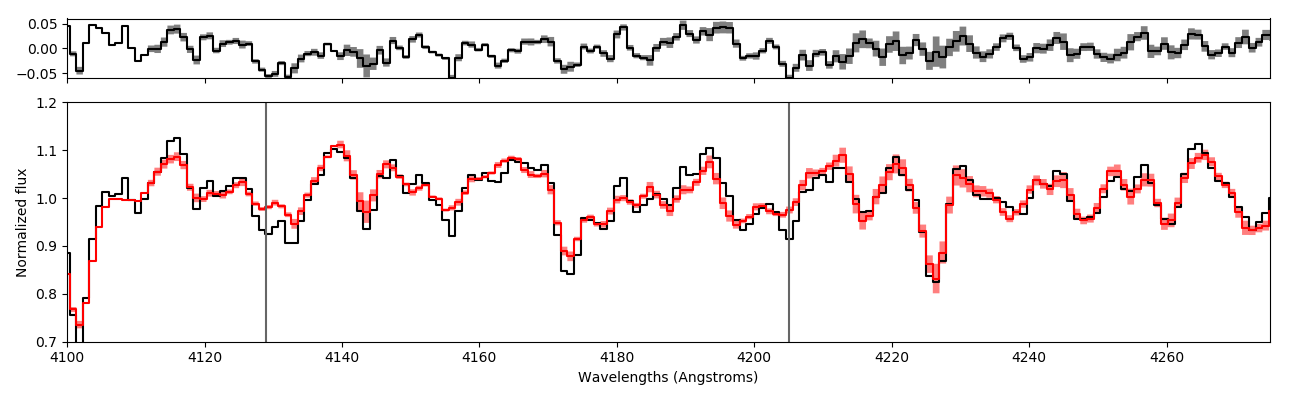
\includegraphics[width=\columnwidth]{423451}
		\caption{The spectral region around two Europium absorption lines at 4129 and 4205 Angstroms. This particular star's spectra (black) shows clear absorption at these wavelengths, as compared to the data-driven model (red).}
		\label{fig:starindex_423451}
	\end{figure}
	
	\begin{figure}
		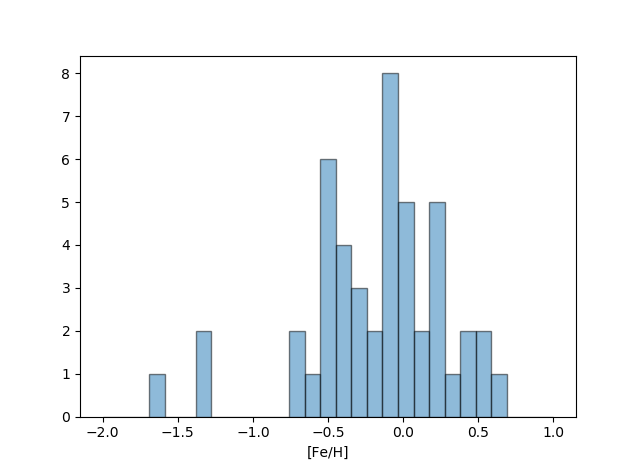
\includegraphics[width=\columnwidth]{metalhistpython}
		\caption{The metallicities of the 47 candidate stars.}
		\label{fig:starindex_423451}
	\end{figure}
	
	\section{Methods}
	
	\subsection{Observations and Candidate Selection}
	
	The LAMOST survey is a low resolution ($R\approx1800$) optical survey that took spectra of stars between 3650-9000 \AA. The second data release from the LAMOST telescope catalogued $\approx$ 2.2 million spectra (low resolution) of stars in the northern sky. Of these 2.2 million, 454,180 giants were fit against a normalised spectra from a sample of 9952 giants \citep{AnnaHo2017}, and from this it became possible to analyse which giants showed an abundance or depletion of particular heavy elements. A machine learning code \textit{The Cannon} was used to fit a predictive model using 9952 LAMOST giant stars that were also found in the higher resolution ($R\approx22500$) APOGEE survey. The labels \textit{The Cannon} predicted were $T_{\rm{eff}}$, $\rm{log_{10}[g]}$, $\rm{[Fe/H]}$, and $\rm{[\alpha/Fe]}$. Normalised spectra was then fit to 454,180 giants from the LAMOST survey and was restricted to between 3905\,\AA\ and 9000\,\AA. For reference, typical uncertainties for these labels are $70\rm{K}$ for $T_{\rm{eff}}$, $0.1$ in $\rm{log_{10}[g]}$, 0.1 in $\rm{[Fe/H]}$, and 0.04 in $\rm{[\alpha/H]}$.
	
	We selected potential candidate stars with an over-abundance of Europium by searching for deviations from the normalized spectra supplied by \textit{The Cannon}. A negative deviation implies an enhancement in a particular element while a positive deviation implies a depletion (compared to what the data-driven model predicted). 
	
	At two absorption lines for Europium (4129\,\AA\ and 4205\,\AA) we fitted Gaussian profiles to each star in the 454,180 giants from LAMOST DR2, and we recorded the amplitude and the wavelength of each, as well as their corresponding errors. Candidate Europium enhanced stars were selected by identifying stars that met the following criteria:
	
	\begin{itemize}
		\item The amplitude of their deviation from the model needed to be less than $\rm{A}<-0.05$;
		\item The signal to noise (S/N) must be greater than 30;
		\item The deviation from the required wavelength in question must be less than 2 \AA;
		\item The reduced $\chi_{\rm{r}}^{2}$ value (where the $\chi_{\rm{r}}^{2}$ value represents how well the model fit the spectrum) must be less than 3, $\chi_{\rm{r}}^{2}<3$.
		\item All of these conditions must be met for both 4129 \AA\ and 4205 \AA\ for us to consider them sufficiently Eu enhanced.
	\end{itemize}   
	
	We gathered an initial sample of 62 candidates out of the 454180 LAMOST giant sample. These were then visually scrutinised to identify those that lacked visual evidence that they were enhanced. After this process we were left with 47 potentially r-process enhanced candidates, 22 of which stand out as very strong candidates.
	
	\section{The r-process}
	For the r-process to occur there must be a very high neutron density, such that neutron capture must be able to occur before the nucleus undergoes a $\beta$-decay (assuming the nucleus is in an unstable state). The conditions that can create this are rare. Events such as supernovae or neutron star mergers list among the most favoured sites.
	
	\subsection{Selection effects}
	The LAMOST giants we analyse belong to a broad range of metallicity ($\rm{[Fe/H]} -1.6\ \rm{to}\ 0.6$), and don't cluster towards any position in the observed sky. These characteristics argue that the abundance we see could not have originated from a common era or site. 
	
	The previous sample of r-process stars, before the release of this letter, almost exclusively consists of metal-poor stars. This fact is not to be confused with saying that most r-process stars found should be metal-poor stars, rather that at low metallicities we know that the s-process will not contribute, so neutron capture elements formed from these stars would be only from the r-process. Over half the current known r-process stars come from a very metal poor ultra faint dwarf galaxy, Reticulum II. However, Europium we know to be totally made from the r-process, therefore even at metallicities where the s-process contributes, Europium is a valuable indication of r-process synthesis.
	
	\subsection{Multiple r-process sites?}
	While it is possible that all currently known r-process enhancements can be made by neutron star mergers, we still have cases of stars in the galaxy which show particularly weak enrichment from r-process elements ([Eu/Fe] < 0.7). These enhancements imply that another site of r-process element synthesis is likely to be active. As we show in \ref{rates}  neutron star merger rates may show that all heavily enriched stars can be enhanced by these phenomena within an adequate time-scale, but we are not able to assume that as a consequence of the merger some stars are greatly enhanced, while others are only very slightly enhanced. It is more accurate to propose that at least two sites exist, with one (potentially mergers) producing a massive amount of enhanced material, and another only producing a small amount, such as supernovae. 
	
	\subsection{Core-collapse supernovae (CCSN)}
	Core-collapse supernova is one of the sites initially proposed to have a high enough neutron density to create elements synthesised by the r-process \citep{Burbidge1957}. 
	
	As of yet our knowledge is incomplete on the exact mechanism that allows material with a high enough neutron density to escape the supernovae event.
	One possible mechanism is the action of high-entropy neutrino winds being released from a proto-neutron star during core-collapse. In this stage of the collapse, this neutrino wind is driving mass loss and could be instrumental in the expulsion of the r-process material in supernovae conditions. However, how much enhanced material is released from the event is very dependant on the amount of material that is allowed to fall back onto the remnant at the arrival of the reverse shock, and so often the supernovae may not release a considerable amount of material \citep{Woosley1992, Burrows1995}. 
	
	Core-collapse supernovae seem to release $M_{\rm{Eu}}\approx10^{-7.5} M_{\odot}$ per event \citep{Argast2004} . While this may not be a particularly significant amount, core-collapse supernovae occur frequently $44700\ \rm{Gpc}^{-3} \rm{yr^{-1}}$ \citep{Li2011}, and so it isn't unreasonable to suggest that, with very little mixing occurring, that much if not all r-process material could have been formed by these and recycled in the stars we present in this letter.
	
	\subsection{Neutron star mergers}
	\label{NSmerg}
	Neutron star mergers are another possible site of r-process element nucleosynthesis \citep{Kasen2017,Hotok2013,Drout2017}. They are easily able to meet the conditions for a high neutron density as interacting tidal forces between the stars rip away neutron dense material allowing r-process element synthesis to occur easily. In this interaction they produce considerably more enriched material than core-collapse supernovae ($M_{\rm{Eu}}\approx10^{-4.5} M_{\odot}$) \citep{Goriely2011}, however the direct interaction and merger of a binary neutron star pair occurs very infrequently with only one ever having been directly observed, and with an upper frequency estimate of $1000\ \rm{Gpc^{-3}yr^{-1}}$ \citep{LIGO2016}. The massive amount of material that these mergers release could more than make up for the low frequency and so, similar to core-collapse supernovae, it is not unreasonable to suggest that they are responsible for most if not all known r-process material. 

	The recent discovery of the UFD Reticulum II \citep{Ji2016} is evidence against the case for a single r-process site. Of nine stars observed in Reticulum II, 7 of them were shown to be highly enriched in r-process elements ($\rm{[Eu/Fe]\approx1.7}$) which suggests a single prolific event having occurred in close proximity to the galaxy early in it's formation, such as a neutron star merger. However, two of the stars observed were only weakly enhanced in r-process elements which suggests that there must have been a second, less efficient, form of r-process enhancement present.
	
	\subsection{The rates of r-process events and what they imply}
	\label{rates}
	From the recent advanced LIGO data \citep{LIGO2016}, we are able to find an estimate for a plausible frequency at which neutron star mergers occur, as mentioned in section \ref{NSmerg}. As well as a reliable estimate of core-collapse supernovae rates from \citet{Li2011}.
	
	From these two rates we can, for the first time to our knowledge, estimate the amount of r-process stars that should be present in the Milky Way, enhanced both by purely neutron star mergers and core-collapse supernovae. We do this assuming instant recycling, and that no r-process matter pollutes stars by any other means than these.
	
	From these rates we can find an estimate of how many r-process enhanced giants should be present from an estimate number of the Milky Way's total stars. As well as an estimate of how many stars, giants or otherwise, should be present in the Milky Way.
	
	In preparing these calculations we assumed a constant star formation rate, 2 M$_\odot yr^{-1}$, in the disk of the Milky Way, $\rm{r=15kpc}$, with a typical IMF and giant star birth rate of approximately $0.3\ $stars per year. We also assumed the lifetime between $\log{g} = 3.2$ and the end of the core-helium burning phase is about $250\,{\rm Myr}$. Therefore if we assume a steady-state system, the number of giant stars in the Milky Way comes to approximately $7.53\times10^7$. This allowed us to find the percentage of the Milky Ways stars that our sample represents.
	
	We also state that a star is said to be enhanced if [Eu/Fe] $\geq$ 0.7, and performed the lower-bound estimate that all of our 47 stars exhibited this abundance. The amount of r-process material expelled is the same as previously discussed, using Europium as our identifier, of $M_{Eu}\approx10^{-4.5} M_{\odot}$.
	
    It was found that in the Milky Way alone there should be present 9,896 r-process enhanced stars. Considering this should be considered a lower-bound estimate (by assuming a lower bound Europium abundance) this is a startlingly large difference from the now updated known amount of r-process enhanced stars which comes to 60. 
    
    Scaling down from the amount of stars in the Milky Way to our sample size of $\approx450000$ giants, the amount of r-process enhanced stars we should find comes to less than one (0.0178). If we are to extend our sample from the 450000 giants, and instead use the entire LAMOST data release 2 (a survey of $\approx2.2$ million stars), we predict that we should still have found less than a single star (0.087)  enhanced in r-process elements. While again this should be considered a lower bound, it is still a startling difference from the 47 that were found.
    
    We can do a similar calculation with our rate of core-collapse supernovae. Taking the same assumptions with minimal mixing, as well as both the ejecta ($M_{Eu}\approx10^{-4.5} M_{\odot}$) and rate ($44700\ \rm{Gpc}^{-3} \rm{yr^{-1}}$) previously discussed, we find that in the Milky Way there should be present 442 r-process enhanced stars made from core-collapse supernovae.
    
    Were we to scale this down to our sample size of $\approx450000$ giants we arrive at a figure of $8.0\times10^{-4}$ stars that should have been observed. Scaling again to the full LAMOST sample we would then expect to find $3.9\times10^{-3}$ enhanced stars. 
    
    From these estimates we can find an approximation for whether or not either neutron star mergers or core-collapse supernovae by themselves are sufficient to enrich our entire r-process enhanced catalogue. 
    
    We find that, by using the assumptions listed, neutron star mergers could create enough r-process material to enrich above the point of [Eu/Fe] > 0.7 for all 60 known r-process enhanced stars within $13.87\times10^9$ years, very close to the age of the universe. From our rates of core-collapse supernovae however, we find that the earliest time-scale at which they can create this level of r-process material is $3.1\times10^{11}$ years, not within the age of the universe. This means with our current knowledge of core-collapse supernovae frequency and the amount of r-process material they eject, there is no way that only core-collapse supernovae could enrich the entire Milky Way.
    
    This is reinforced by the enhanced stars found in the LAMOST sample. 47 is greater than 10\% of all enhanced stars that should be present in the Milky Way according to the solely core-collapse supernovae rate. However, the LAMOST data release 2 only surveyed 0.00088\% of the Milky Way. The idea that over 10\% of all r-process stars were found in this small a percentage is improbable, and so we can say that core-collapse supernovae can not be the only source of r-process material. 
    
    \todo{For Andy (haven't written this bit nicely this was a thought dump): Let us consider that both of these estimates are correct, and the rates they are based on have been roughly accurate over the age of the universe (although they should have increased with time, which is actually a bit worse for us). Then we are left with our previous prediction of 9,896 stars enhanced purely by neutron star mergers, and another 442 stars enhanced purely by core-collapse supernovae. This leaves us with a new sample of r-process enhanced stars that should exist in the Milky Way of 10,338. 
    At a rough estimate, the LAMOST data release 2 took spectra for 0.00088\% of the Milky Way's stars (assuming an average amount of stars in the Milky Way of 250 billion). In this very small percentage, 47 r-process enhanced stars were found. Then, if we are able to assume that there is nothing particularly special about the area of the sky that LAMOST surveyed, scaling this size to that of the Milky Way we should find 5,340,892 r-process enhanced stars. Clearly there is something wrong.}
    
	
	\section{Conclusions}
	We present the largest to date sample of r-process element enhanced stars. These stars are found at a wide range of metallicities, contrary to previous discoveries that focussed on metal-poor r-process enhanced stars. Similarly they are not clumped in either temperatures, $log(g)$, or radial velocity. They don't cluster to any one end of the H-R diagram, so it is likely there is no correlation between type of star. They are found both in the disk and halo, and are not clustered anywhere in the sky. In addition to this we also present the first ever estimate to our knowledge, from information provided by advanced LIGO, that neutron star mergers possess the ability to synthesise all currently known r-process material in a feasible time-scale. We also provide evidence that we are confident to say means that core-collapse supernovae can not possibly be the only progenitors of r-process material in the Milky Way Galaxy.
	
	We recommend follow-up high resolution spectra be obtained for each of the 47 stars to ascertain how enhanced they are. To find the origin of these stars and to show whether or not they may come from a similar progenitor site it is necessary to find orbits for them.
	
	
	% The best way to enter references is to use BibTeX:
	
	\bibliographystyle{mnras}
	%\bibliography{paper} % if your bibtex file is called example.bib
	\begin{thebibliography}{99}
		\bibitem[\protect\citeauthoryear{Sneden, C. et al.}{2008}]{Sneden2008}
		Sneden C., Cowan J.J., \& Gallino R. 2013, Annual review of Astronomy \& Astrophysics, 46, 1
		\bibitem[\protect\citeauthoryear{Ji, A. P. et al.}{2016}]{Ji2016}
		Ji A. P., Frebel A., Chiti A., \& Simon J. D. 2016, Nature, 531
		\bibitem[\protect\citeauthoryear{Ho et al.}{2017}]{AnnaHo2017}
		Ho A. Y. Q., Ness M. K., Hogg David W., Rix H-W., Liu C., Yang F., Zhang Y., Hou Y.,\& Wang Y. 2017, ApJ, 836, 1
		\bibitem[\protect\citeauthoryear{Burbidge, E. et al.}{1957}]{Burbidge1957}
		Burbidge E. M., Burbidge G. R., Fowler W. A., \& Hoyle F. 1957, Review of Modern Physics, 29, 4
		\bibitem[\protect\citeauthoryear{Goriely, S. et al.}{2011}]{Goriely2011}
		Goriely S., Bauswein A. \& Janka H-T. 2011, , 738, L32
		\bibitem[\protect\citeauthoryear{Abbott, B.P. et al.}{2016}]{LIGO2016}
		Abbot B.P. et al. 2016, Living Reviews in Relativity, 19, 1
		\bibitem[\protect\citeauthoryear{Argast, D. et al.}{2004}]{Argast2004}
		Argast D., Samland M., Thielmann F-K. \& Qian Y-Z. 2004, Astronomy and Astrophysics, 416
		\bibitem[\protect\citeauthoryear{Woosley, S.E. et al.}{1992}]{Woosley1992}
		Woosley S.E, \& Hoffman R.D. 1992, ApJ, 395, 1
		\bibitem[\protect\citeauthoryear{Burrows, A. et al.}{1995}]{Burrows1995}
		Burrows, A., Hayes, J., \& Fryxell, Bruce A. 1992, ApJ, 450, 830
		\bibitem[\protect\citeauthoryear{Li, W. et al.}{2011}]{Li2011}
		Li, W., Chornock, R., Leaman, J., Filippenko, A. V., Poznanski, D., Wang, X., Ganshalingam, M., \& Mannucci, F. 2011, Royal Astronomical Society, 412, 1473
		\bibitem[\protect\citeauthoryear{Drout, M. R. et al.}{2017}]{Drout2017}
		Drout, M. R. et al. 2017, Science
		\bibitem[\protect\citeauthoryear{Kasen, D. et al.}{2017}]{Kasen2017}
		Kasen, D., Metzger, B., Barnes, J., Quataert, E., \& Ramirez-Ruiz, E. 2017, Nature, 551, 7678
		\bibitem[\protect\citeauthoryear{Hotokezaka, K. et al.}{2013}]{Hotok2013}
		Hotokezaka, K., Kiuchi, K., Kyutoku, K., Okawa, H., Skiguchi, Y., Shibata, M., \& Taniguchi, K. 2013, APS
	\end{thebibliography}
	
	% Please add the following required packages to your document preamble:
	% \usepackage{booktabs}
	% Please add the following required packages to your document preamble:
	% \usepackage{booktabs}
	\begin{table*}
		\centering
		\label{Data for the 47}
		\begin{tabular}{@{}cccccccccccc@{}}
			\toprule
			\textbf{2MASS ID}   & \textbf{RA} & \textbf{DEC} & \textbf{S/N}        	& \textbf{$\boldsymbol{V_{\rm{r}}}$}   & \textbf{$\boldsymbol{T_{\rm{eff}}}$} & \textbf{Log(g)}	& \textbf{$\boldsymbol{[\rm{Fe/H}]}$} & \textbf{$\boldsymbol{[\alpha/\rm{H}]}$} & \textbf{$\boldsymbol{\chi_{\rm{r}}^{2}}$} & \textbf{{[}Eu/Fe{]}} & \textbf{Error} \\
			-               	& {[}deg{]}   & {[}deg{]}	& {[}$\rm{pixel}^{-1}${]} & {[}$\rm{km\ s}^{-1}${]} & {[}K{]}             	& {[}$cm\ s^{-2}${]} & {[}dex{]}          	& {[}dex{]}              	& -                        	& {[}dex{]}        	& {[}dex{]}  	\\ \midrule
			J130303.65+260837.0 & 13:03:03.65 & +26:08:37.0  & 36.48               	& -37.77              	& 4851.24             	& 2.98           	& -0.54              	& 0.19                   	& 0.42                     	& 1.39             	& 0.31       	\\
			J062733.76+280814.1 & 06:27:33.77 & +28:08:14.2  & 39.08               	& 38.67               	& 4502.58             	& 1.92           	& -0.15              	& 0.00                   	& 0.35                     	& 1.43             	& 0.35       	\\
			J070035.19+103443.5 & 07:00:35.19 & +10:34:43.5  & 41.77               	& 17.69               	& 4752.08             	& 2.44           	& -0.43              	& 0.06                   	& 0.33                     	& 1.09             	& 0.63       	\\
			J070107.18+125948.2 & 07:01:07.19 & +12:59:48.2  & 33.72               	& 46.17               	& 4452.61             	& 2.51           	& 0.47               	& 0.02                   	& 0.36                     	& 1.30             	& 0.31       	\\
			J063400.95+420904.3 & 06:34:00.96 & +42:09:04.4  & 34.09               	& 9.89                	& 4315.56             	& 1.62           	& -0.50              	& 0.10                   	& 0.43                     	& 1.19             	& 3.10       	\\
			J220118.66+033558.6 & 22:01:18.66 & +03:35:58.6  & 35.11               	& -108.23             	& 4790.06             	& 2.51           	& -1.36              	& 0.33                   	& 0.37                     	& 1.44             	& 0.26       	\\
			J221220.27+032735.4 & 22:12:20.27 & +03:27:35.5  & 35.16               	& -12.89              	& 4867.34             	& 3.12           	& 0.11               	& 0.14                   	& 0.35                     	& 1.52             	& 0.20       	\\
			J060021.29+384840.6 & 06:00:21.29 & +38:48:40.6  & 30.03               	& 32.68               	& 4305.08             	& 2.10           	& 0.15               	& -0.01                  	& 0.54                     	& 1.49             	& 0.35       	\\
			J081632.10-053703.4 & 08:16:32.11 & -05:37:03.4  & 59.16               	& 44.67               	& 4541.14             	& 2.45           	& 0.57               	& 0.03                   	& 0.75                     	& 1.34             	& 0.26       	\\
			J064641.14+235318.2 & 06:46:41.14 & +23:53:18.3  & 36.77               	& 25.78               	& 4325.56             	& 1.78           	& -0.10              	& 0.02                   	& 0.42                     	& 1.41             	& 0.27       	\\
			J025225.88+324308.1 & 02:52:25.88 & +32:43:08.2  & 34.79               	& 24.88               	& 4797.58             	& 2.52           	& -0.23              	& 0.05                   	& 0.24                     	& 1.31             	& 0.29       	\\
			J061822.02+015126.7 & 06:18:22.02 & +01:51:26.8  & 36.75               	& 45.27               	& 4617.95             	& 2.43           	& -0.12              	& 0.04                   	& 0.34                     	& 1.42             	& 0.30       	\\
			J083049.21+304144.3 & 08:30:49.21 & +30:41:44.3  & 39.5                	& -125.31             	& 4859.92             	& 2.28           	& -1.63              	& 0.33                   	& 0.41                     	& 1.52             	& 0.20       	\\
			J035949.12+302104.4 & 03:59:49.13 & +30:21:04.4  & 30.42               	& 26.98               	& 4164.41             	& 1.79           	& -0.12              	& 0.00                   	& 0.36                     	& 1.47             	& 0.32       	\\
			J074852.24+075016.5 & 07:48:52.25 & +07:50:16.6  & 33.47               	& 36.87               	& 4405.84             	& 1.94           	& -0.48              	& 0.07                   	& 0.30                     	& 1.44             	& 0.30       	\\
			J163116.81+002349.5 & 16:31:16.81 & +00:23:49.5  & 32.63               	& -35.98              	& 4628.92             	& 2.53           	& 0.01               	& 0.18                   	& 0.29                     	& 1.44             	& 0.32       	\\
			J073532.54+215850.0 & 07:35:32.55 & +21:58:50.0  & 35.61               	& 35.98               	& 4859.66             	& 3.27           	& 0.19               	& 0.06                   	& 0.44                     	& 1.19             	& 0.79       	\\
			J164023.01+164552.5 & 16:40:23.02 & +16:45:52.6  & 44.59               	& -34.18              	& 4964.91             	& 2.96           	& 0.36               	& 0.07                   	& 0.35                     	& 1.27             	& 0.32       	\\
			J153333.12+510621.8 & 15:33:33.13 & +51:06:21.9  & 49.45               	& -17.99              	& 4861.78             	& 2.51           	& -0.49              	& 0.22                   	& 0.46                     	& 1.31             	& 0.28       	\\
			J175737.71+521523.1 & 17:57:37.71 & +52:15:23.2  & 38.52               	& -40.47              	& 4861.38             	& 3.36           	& -0.34              	& 0.10                   	& 0.55                     	& 1.51             	& 0.24       	\\
			J184125.86+432807.8 & 18:41:25.86 & +43:28:07.9  & 46.94               	& -93.84              	& 4703.92             	& 2.61           	& -0.26              	& 0.27                   	& 0.33                     	& 1.20             	& 0.34       	\\
			J195234.41+470859.4 & 19:52:34.41 & +47:08:59.5  & 68.57               	& -24.28              	& 4596.44             	& 2.54           	& 0.55               	& 0.07                   	& 0.82                     	& 0.95             	& 0.48       	\\
			J215146.68+304016.0 & 21:51:46.68 & +30:40:16.0  & 73.25               	& -28.78              	& 4566.21             	& 2.48           	& 0.64               	& 0.04                   	& 0.71                     	& 0.88             	& 0.45       	\\
			J075116.55+220137.8 & 07:51:16.56 & +22:01:37.9  & 32.87               	& 90.24               	& 4810.60             	& 2.70           	& -0.33              	& 0.02                   	& 0.30                     	& 1.35             	& 0.31       	\\
			J003929.43+430039.5 & 00:39:29.43 & +43:00:39.6  & 33.14               	& -104.33             	& 4190.26             	& 1.87           	& -0.01              	& 0.07                   	& 0.41                     	& 1.35             	& 0.33       	\\
			J040122.07+461504.5 & 04:01:22.08 & +46:15:04.5  & 35.43               	& -95.03              	& 4305.88             	& 1.75           	& 0.02               	& 0.10                   	& 0.57                     	& 1.37             	& 0.35       	\\
			J040815.45+464920.1 & 04:08:15.46 & +46:49:20.1  & 33.05               	& 16.19               	& 4855.16             	& 2.65           	& -0.11              	& 0.00                   	& 0.30                     	& 1.48             	& 0.30       	\\
			J071206.83+213038.0 & 07:12:06.84 & +21:30:38.1  & 32.66               	& 29.08               	& 4432.03             	& 1.75           	& -0.38              	& 0.11                   	& 0.40                     	& 1.47             	& 0.28       	\\
			J222820.22+340750.3 & 22:28:20.22 & +34:07:50.3  & 34.52               	& -45.27              	& 4419.96             	& 2.06           	& -0.07              	& 0.11                   	& 0.49                     	& 1.37             	& 0.31       	\\
			J222310.49+344357.4 & 22:23:10.50 & +34:43:57.5  & 54.06               	& -20.09              	& 4232.66             	& 1.87           	& -0.01              	& 0.03                   	& 0.86                     	& 1.22             	& 0.31       	\\
			J222101.61+365923.6 & 22:21:01.62 & +36:59:23.7  & 30.81               	& -27.88              	& 4360.28             	& 2.23           	& 0.20               	& 0.04                   	& 0.45                     	& 1.47             	& 0.29       	\\
			J052327.44+571126.8 & 05:23:27.45 & +57:11:26.8  & 33.54               	& -24.88              	& 4806.24             	& 3.08           	& 0.24               	& 0.07                   	& 0.45                     	& 1.43             	& 0.25       	\\
			J235212.27+492548.4 & 23:52:12.27 & +49:25:48.4  & 39.93               	& -95.03              	& 5047.36             	& 3.30           	& -0.43              	& 0.22                   	& 0.29                     	& 1.28             	& 0.26       	\\
			J074102.63+130520.3 & 07:41:02.64 & +13:05:20.4  & 40.83               	& 49.17               	& 5000.84             	& 3.00           	& -0.38              	& -0.02                  	& 0.30                     	& 1.35             	& 0.27       	\\
			J061559.10+470344.9 & 06:15:59.11 & +47:03:44.9  & 36.84               	& -18.29              	& 4811.98             	& 2.82           	& -0.59              	& 0.07                   	& 0.44                     	& 1.00             	& 1.33       	\\
			J054704.12+600827.1 & 05:47:04.13 & +60:08:27.1  & 33.19               	& -23.33              	& 4770.80             	& 2.64           	& -0.10              	& 0.06                   	& 0.40                     	& 1.46             	& 0.26       	\\
			J055548.33+611537.1 & 05:55:48.33 & +61:15:37.1  & 33.6                	& -40.88              	& 4850.39             	& 2.57           	& -0.46              	& 0.13                   	& 0.22                     	& 1.42             	& 0.26       	\\
			J042723.73+271546.8 & 04:27:23.73 & +27:15:46.9  & 45.73               	& -40.17              	& 4211.91             	& 1.72           	& -0.04              	& 0.05                   	& 0.79                     	& 1.33             	& 0.34       	\\
			J035702.05+281335.2 & 03:57:02.06 & +28:13:35.3  & 31.82               	& -44.67              	& 4712.89             	& 2.44           	& 0.01               	& 0.16                   	& 0.46                     	& 1.28             	& 0.38       	\\
			J031030.13+531759.9 & 03:10:30.13 & +53:17:59.9  & 35.34               	& -16.79              	& 4699.75             	& 2.34           	& 0.21               	& 0.00                   	& 0.89                     	& 1.51             	& 0.21       	\\
			J091256.32+353008.3 & 09:12:56.32 & +35:30:08.3  & 73.39               	& 20.39               	& 4441.95             	& 2.33           	& 0.41               	& 0.02                   	& 0.76                     	& 0.92             	& 0.39       	\\
			J071534.00+211353.8 & 07:15:34.00 & +21:13:53.9  & 31.68               	& 42.27               	& 4892.00             	& 2.57           	& -0.72              	& 0.11                   	& 0.34                     	& 0.59             	& 0.29       	\\
			J101317.14+122928.8 & 10:13:17.14 & +12:29:28.8  & 45.54               	& 300.69              	& 5055.95             	& 2.24           	& -1.34              	& 0.33                   	& 0.38                     	& 1.46             	& 0.24       	\\
			J161326.00+073218.1 & 16:13:26.00 & +07:32:18.2  & 48.45               	& -50.07              	& 5086.79             	& 3.40           	& -0.68              	& 0.29                   	& 0.93                     	& 1.38             	& 0.24       	\\
			J173711.85+101126.6 & 17:37:11.85 & +10:11:26.7  & 30.01               	& -33.58              	& 4991.07             	& 3.49           	& -0.05              	& 0.17                   	& 0.41                     	& 1.45             	& 0.28       	\\
			J173041.92+125640.5 & 17:30:41.92 & +12:56:40.5  & 52.67               	& 20.39               	& 4986.98             	& 3.42           	& -0.45              	& 0.22                   	& 0.30                     	& 1.09             	& 0.43       	\\
			J172929.42+120133.3 & 17:29:29.43 & +12:01:33.3  & 39.91               	& 14.39               	& 4597.08             	& 2.67           	& 0.24               	& 0.05                   	& 0.67                     	& 1.02             	& 0.80       	\\ \bottomrule
		\end{tabular}
		\caption{Abundances and additional information of the 47 enhanced stars.}
	\end{table*}
	
	
	
	
	
	% Don't change these lines
	%\bsp	% typesetting comment
	\label{lastpage}
\end{document}
